\documentclass[12pt,a4paper]{article}
\usepackage[utf8]{inputenc}
\usepackage{pdfpages}
\usepackage[magyar]{babel}
\usepackage{hyperref}	
\hypersetup{					
colorlinks=false,						
pdfborder={0 0 0},
}
\usepackage{fancyhdr}
\usepackage[left=2cm,right=2cm,top=3.5cm,bottom=3cm,headsep=50pt]{geometry}

\begin{document}
%=================================================
\thispagestyle{empty}
\begin{center}

\includegraphics[scale=0.3]{bme.pdf}\\
\large{Budapesti Műszaki- és Gazdaságtudományi Egyetem\\
Gépészmérnöki kar}\\[1cm]
\begin{Huge}
\textbf{Mechatronika projekt}
\end{Huge}\\[0.5cm]

\Large{BMEGEFOAMM3}\\[2cm]
\Huge{\bf{3D szkenner}}\\[2.5cm]
\bf{\Large{Tar Dániel\\[5pt]
		Bognár Máté\\
		Varga Roland}}\\[1cm]


\includegraphics[scale=0.5]{mogilogo.jpg}\\[1cm]
\large{\today}
\end{center}
%=================================================
\newpage
\tableofcontents
\newpage
\pagestyle{fancy}
\fancyhf{}
\rhead{Tar Dániel\\Bognár Máté\\Varga Roland}
\lhead{3D szkenner}
\cfoot{\thepage. oldal}
%=================================================
\section{Bevezető}
Az iparban egyre elterjedtebb a 3D szkennerek alkalmazása. Jól használhatóak gyors prototípuskészítésre és `'reverse engineering'' eljárásokhoz. Ezzel jelentős modellezési és mérési idő takarítható meg.\\[10pt]
Új eszközök tervezésénél és komplex alkatrészek méreteinek gyors meghatározására egyaránt használható. Apróbb mechanikai alkatrészek, turbinalapátok és helységek szkennelése is lehetséges adott felbontással.\\[10pt]
A gyógyászatban alkalmazzák például test vagy testrész modellezésére, mivel egyes protézisek elkészítése nagy méretpontosságot igényel, és így könnyebben formálhatóak az egyéni igények szerint.\\[10pt]
Egyetemeken régészek is használhatják leletek tanulmányozására anélkül, hogy bármilyen kártétel veszélye fennállna.\\[10pt]
\begin{figure}[h!]
\centering
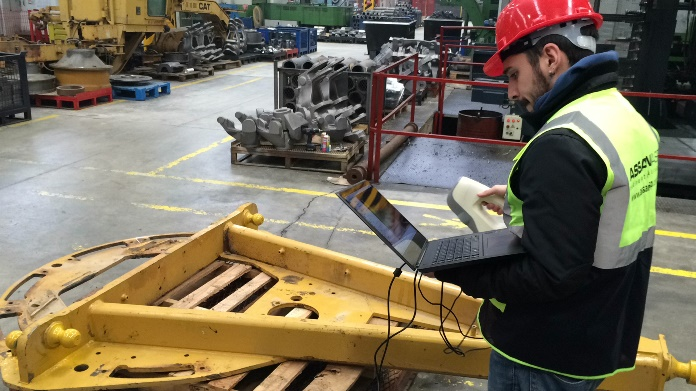
\includegraphics[height=5cm]{images/application1.jpg}
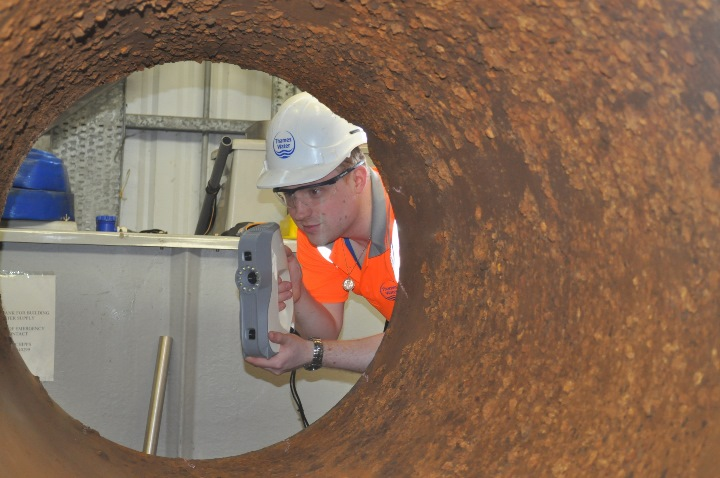
\includegraphics[height=5cm]{images/application2.jpg}
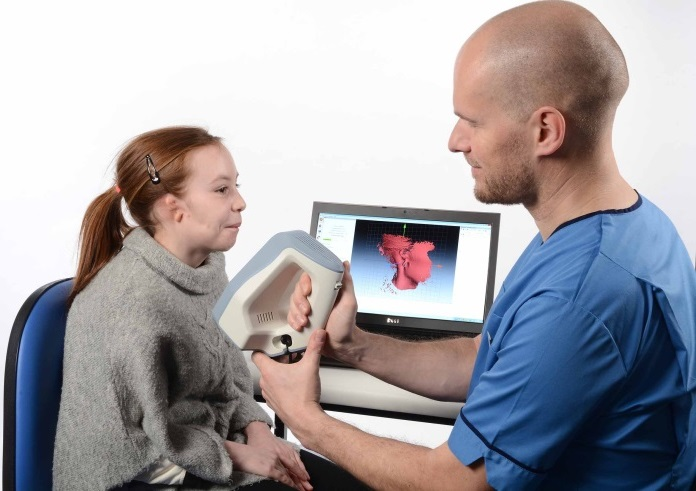
\includegraphics[height=5cm]{images/application3.jpg}
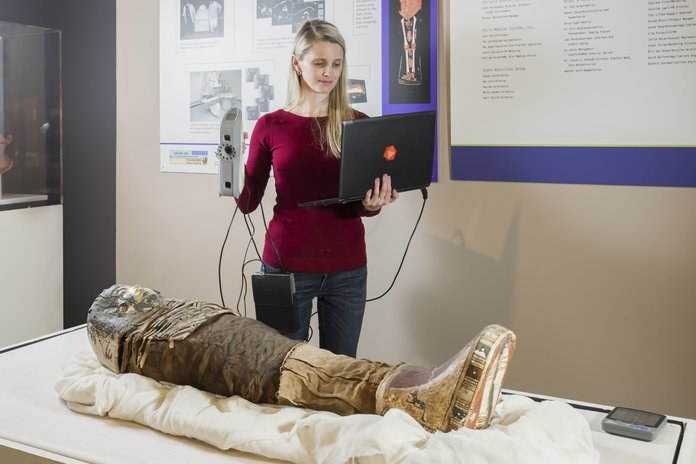
\includegraphics[height=5cm]{images/application4.jpg}
\caption{3D szkenner alkalmazása a hétköznapokban\cite{alkalmazasok}}
\end{figure}
%=================================================
\newpage
\section{Feladat leírása}
\subsection{Követelmények}
A projekt célja egy használható 3D lézerszkenner eljárás kidolgozása és megvalósítása, ami az alábbi követelményeknek megfelel:
\begin{enumerate}
	\item A konstrukció hordozhatósága: viszonylag kis befoglaló mérettel kell 			rendelkezzen és könnyen szétszerelhető-összerakható legyen.\label{hordozhatosag}
	\item A szerkezet legyen alkalmas a szerkezet együttes szabványos fényképezőállványra való rögzítésére.\label{kameraallvanyra}
	\item A megírt program átláthatóságára (felhasználóbarát) és jól dokumentáltságára kell törekedni, hogy a projektet a későbbiekben mások is tovább tudják vinni.\label{felhasznalobarat}
\end{enumerate}
\subsection{Alap koncepció}
A szkennelési módszert egy webkamera, egy vonallézer és egy forgóasztal felhasználásával dolgoztuk ki. Az eljárás lényege, hogy a tárgyra vetült lézerfény vonalról a kamerával valamekkora szögből kép készül. A képen a forgóasztal forgástengelyének meghatározhatónak kell lennie, és ez a vonallézer által meghatározott síkba kell hogy essen. A lézerpontok forgástengelytől (és azon egy tetszőleges origótól) vett távolságából a térbeli helyzetük meghatározható.
%=================================================
\section{Alapul vett szakirodalom} % -  tard
%=================================================
	%"3d laserscanner" kulcsszót beírva a Google-be rengeteg találatot kap az ember. Mi elsőnek a képi és videó találatokat %nézegettük meg, és rögtön megállapítottuk, hogy nagyon menő lesz az általunk készített kis kütyü / szerkezet.\\
	
	Alapvetően kétféle lézer szkenner található meg a piacon. Az egyik, ami az adott tárgyat, objektumot végigpásztázza egy lézerfény segítségével és a lézerfény kibocsájtásától, a lézerfény visszaérkezéséig eltelt időből számítja a távolságot. Ez egy elég drága technika, mivel nagyon pontosan kell mérni az időt, mivel a fény terjedési sebessége nagyon nagy, ezért körülbelül $[ns]$ nagyságrendben kell mérni az idő múlását.
	\\
	\begin{figure}[h!]
		\begin{center}
			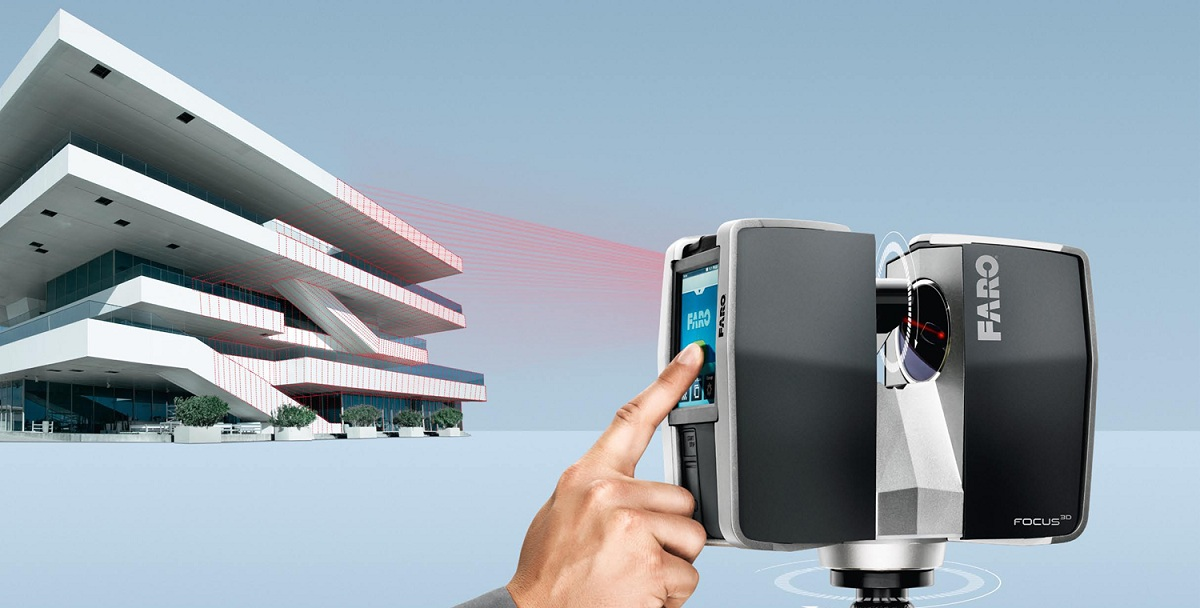
\includegraphics[height=5cm]{images/Faro_Building_Scan}
			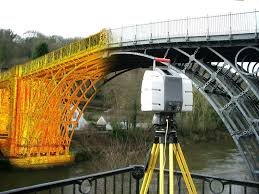
\includegraphics[height=5cm]{images/Bridge_Scan}
		\end{center}
		\caption{Távolságmérésen alapuló lézerszkenner\cite{FaroBuildingScan}\cite{BridgeScan}}
	\end{figure}

	A másik, ami egy vonallézerrel világítja meg a tárgy felületét, majd képfeldolgozással felismerve a megvilágított élt, különböző módszerek alapján, előállít egy pontfelhőt. A pontfelhőből háromszögeléses technikával pedig elkészít egy felületmodellt.
	\\
	
	\begin{figure}[h!]
		\begin{center}
			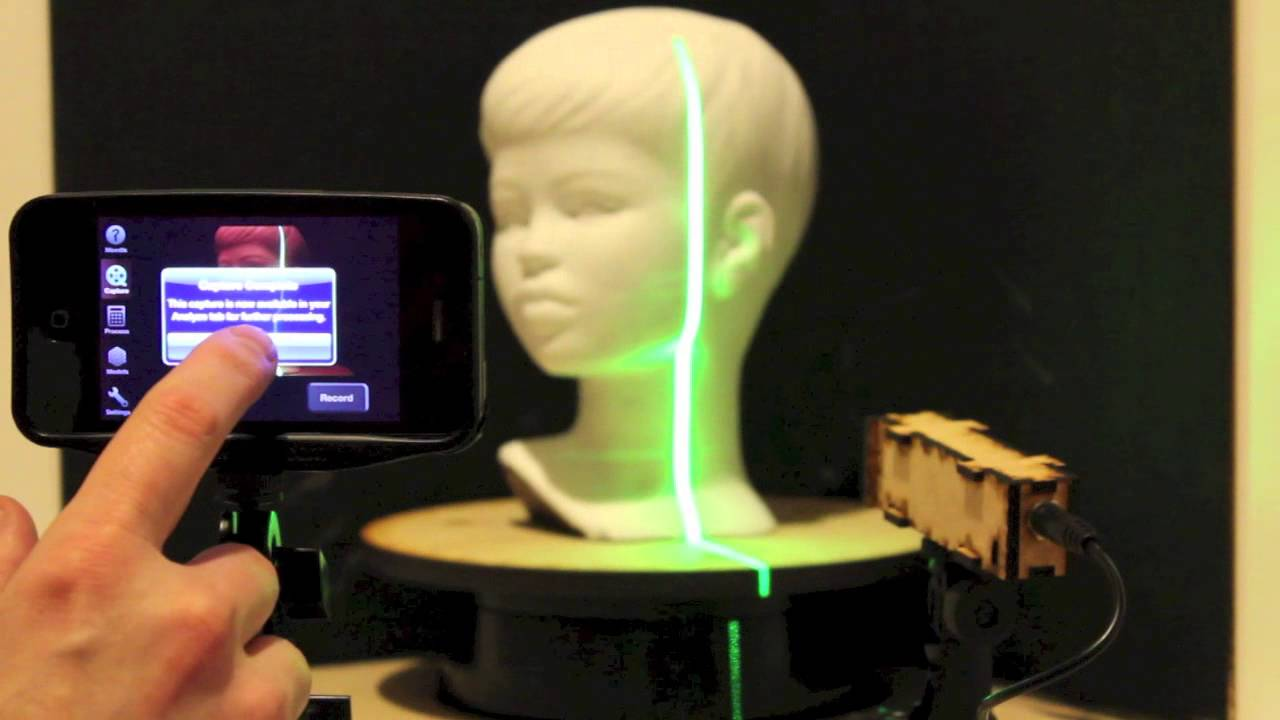
\includegraphics[height=5cm]{images/Mobile_Scan}
			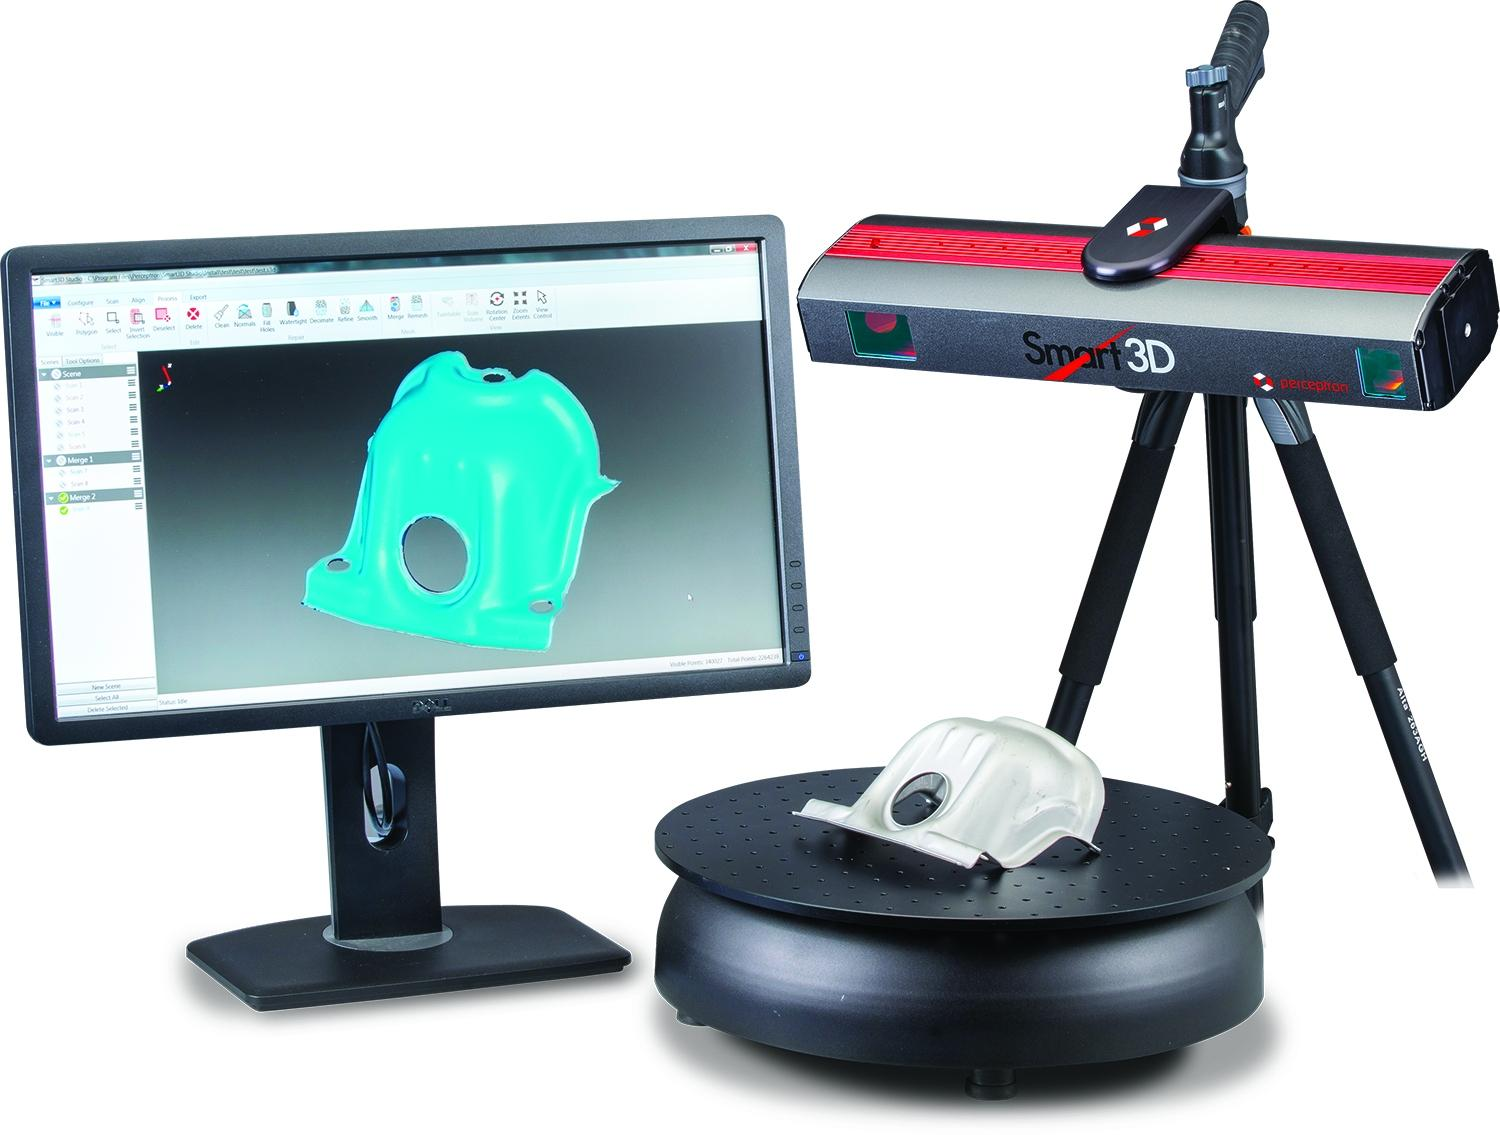
\includegraphics[height=5cm]{images/PC_Scan}
		\end{center}
		\caption{Forgóasztalos, képfeldolgozáson alapuló\cite{MobileScan}\cite{PCScan}}
	\end{figure}

	A rendelkezésre álló eszközök, a feladatleírás és a költségek alapján a második módszert választottuk. A projekt kiindulása képpen nagy segítségünkre volt az \href{http://www.instructables.com/id/3D-Laser-Scanning-DIY/}{\textit{Instructables}} oldalon található \textit{DIY: How to Make a Low Cost 3D Scanner}\cite{LaserScannerProjekt} nevű projekt. Ez adott alapot a gondolkodásmódunknak, de végül teljesen más módszerrel dolgozzuk fel az adatokat.

%=================================================
\section{Felhasznált hardverek}
\subsection{Beszerzett eszközök}
A projektfeladat már az előző évben is ki volt adva, a tavalyi csoportnak ugyan nem sikerült befejeznie, de néhány általuk készített alkatrész öröklődött. Így már kézhez kaptuk egy  LFL650-5-12(9x20)60-as típusú vonallézert,
egy unipoláris léptető motort, a tanszéki KUTESZ alkatrészekből összeállított állvánnyal és egy kisebb méretű asztallal,
illetve a motor meghajtó áramkört is.
\\[10pt]
A felhasznált hardverek egy másik része Bojtos Attila tanár úrtól származik. Ilyen a fényképezőgép állvány, az erre később rögzített 20x20-as ITEM-5-ös profil, és egy Canyon márkájú, 640x480-as felbontású webkamera.
\\[10pt]
Általunk beszerzett alkatrész még a forgóasztalt vezérlő áramkör: ...
És a lézert kapcsoló egység: ...
 \begin{figure}[h!]
 	\centering
 	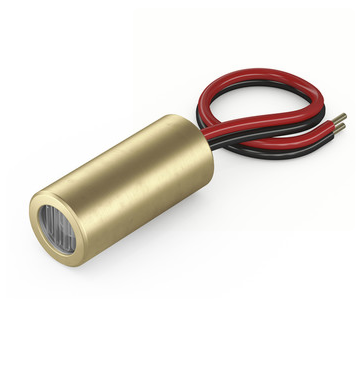
\includegraphics[scale=0.5]{images/laser}
 	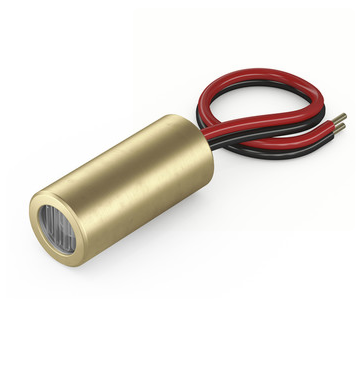
\includegraphics[scale=0.5]{images/laser}
	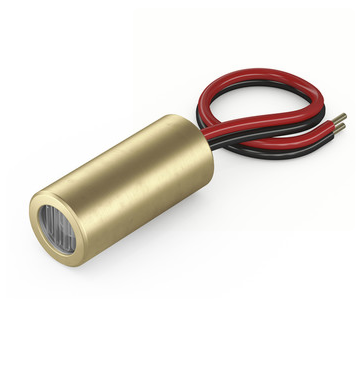
\includegraphics[scale=0.5]{images/laser}
	\caption{Beszerzett eszközök}
\end{figure}

\subsection{Saját készítésű eszközök}
Az általunk tervezett alkatrészek többsége 3D nyomtatással készült, ezek a kamerát és lézert az ITEM profilra rögzítő elemek. A lézer lefogó, amely a lézert rögzíti a profil közepén. És a kamera tartó, ami két alkatrész közé szorítja be a kamera alsó részét, a gyári foglalathoz hasonló módon.\\[10pt]
Emellett a követelményeknek megfelelő szkennelhető tárgyméret miatt tervezni kellett egy új forgóasztalt. Ez az asztal 180mm átmérőjű, központosító körökkel ellátott, a KUTESZ elemekkel kompatibilis furatkiosztású elem.
Végül a profilt a kamera állványra rögzítő elem egy 6mm vastag,  lemez alkatrész.
 \begin{figure}[h!]
 	\centering
	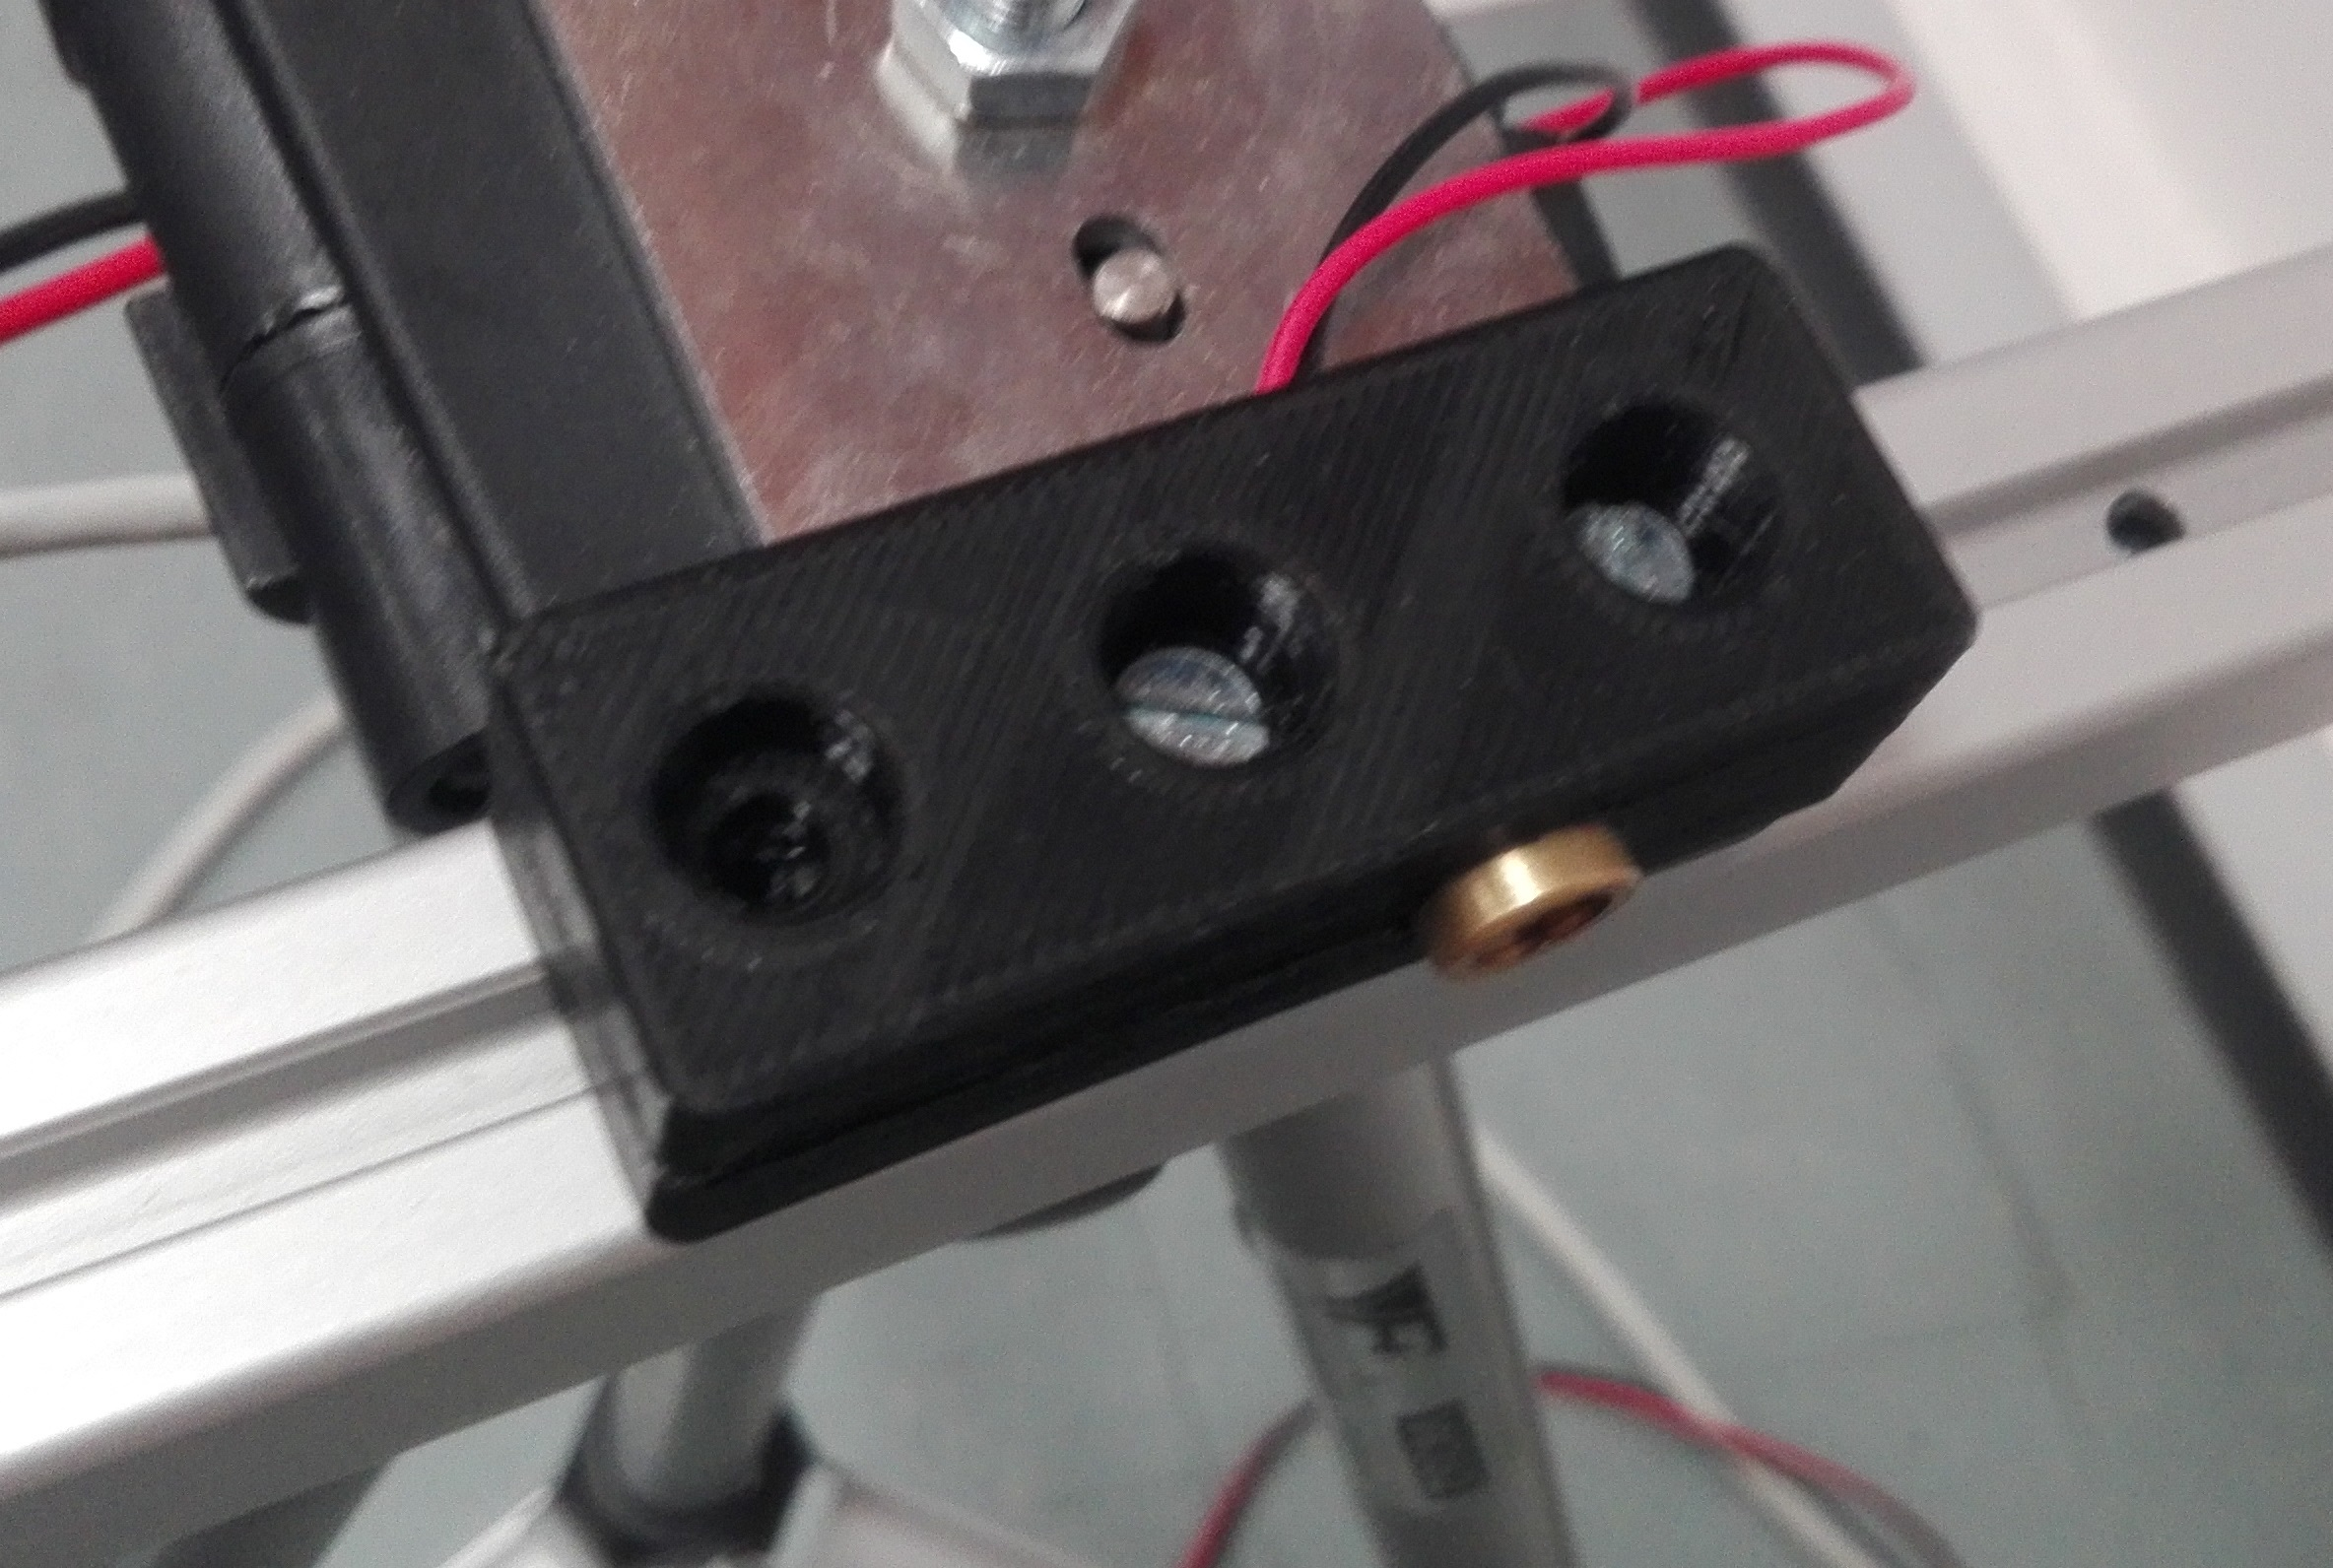
\includegraphics[height=5cm]{images/lezerlefogo}
	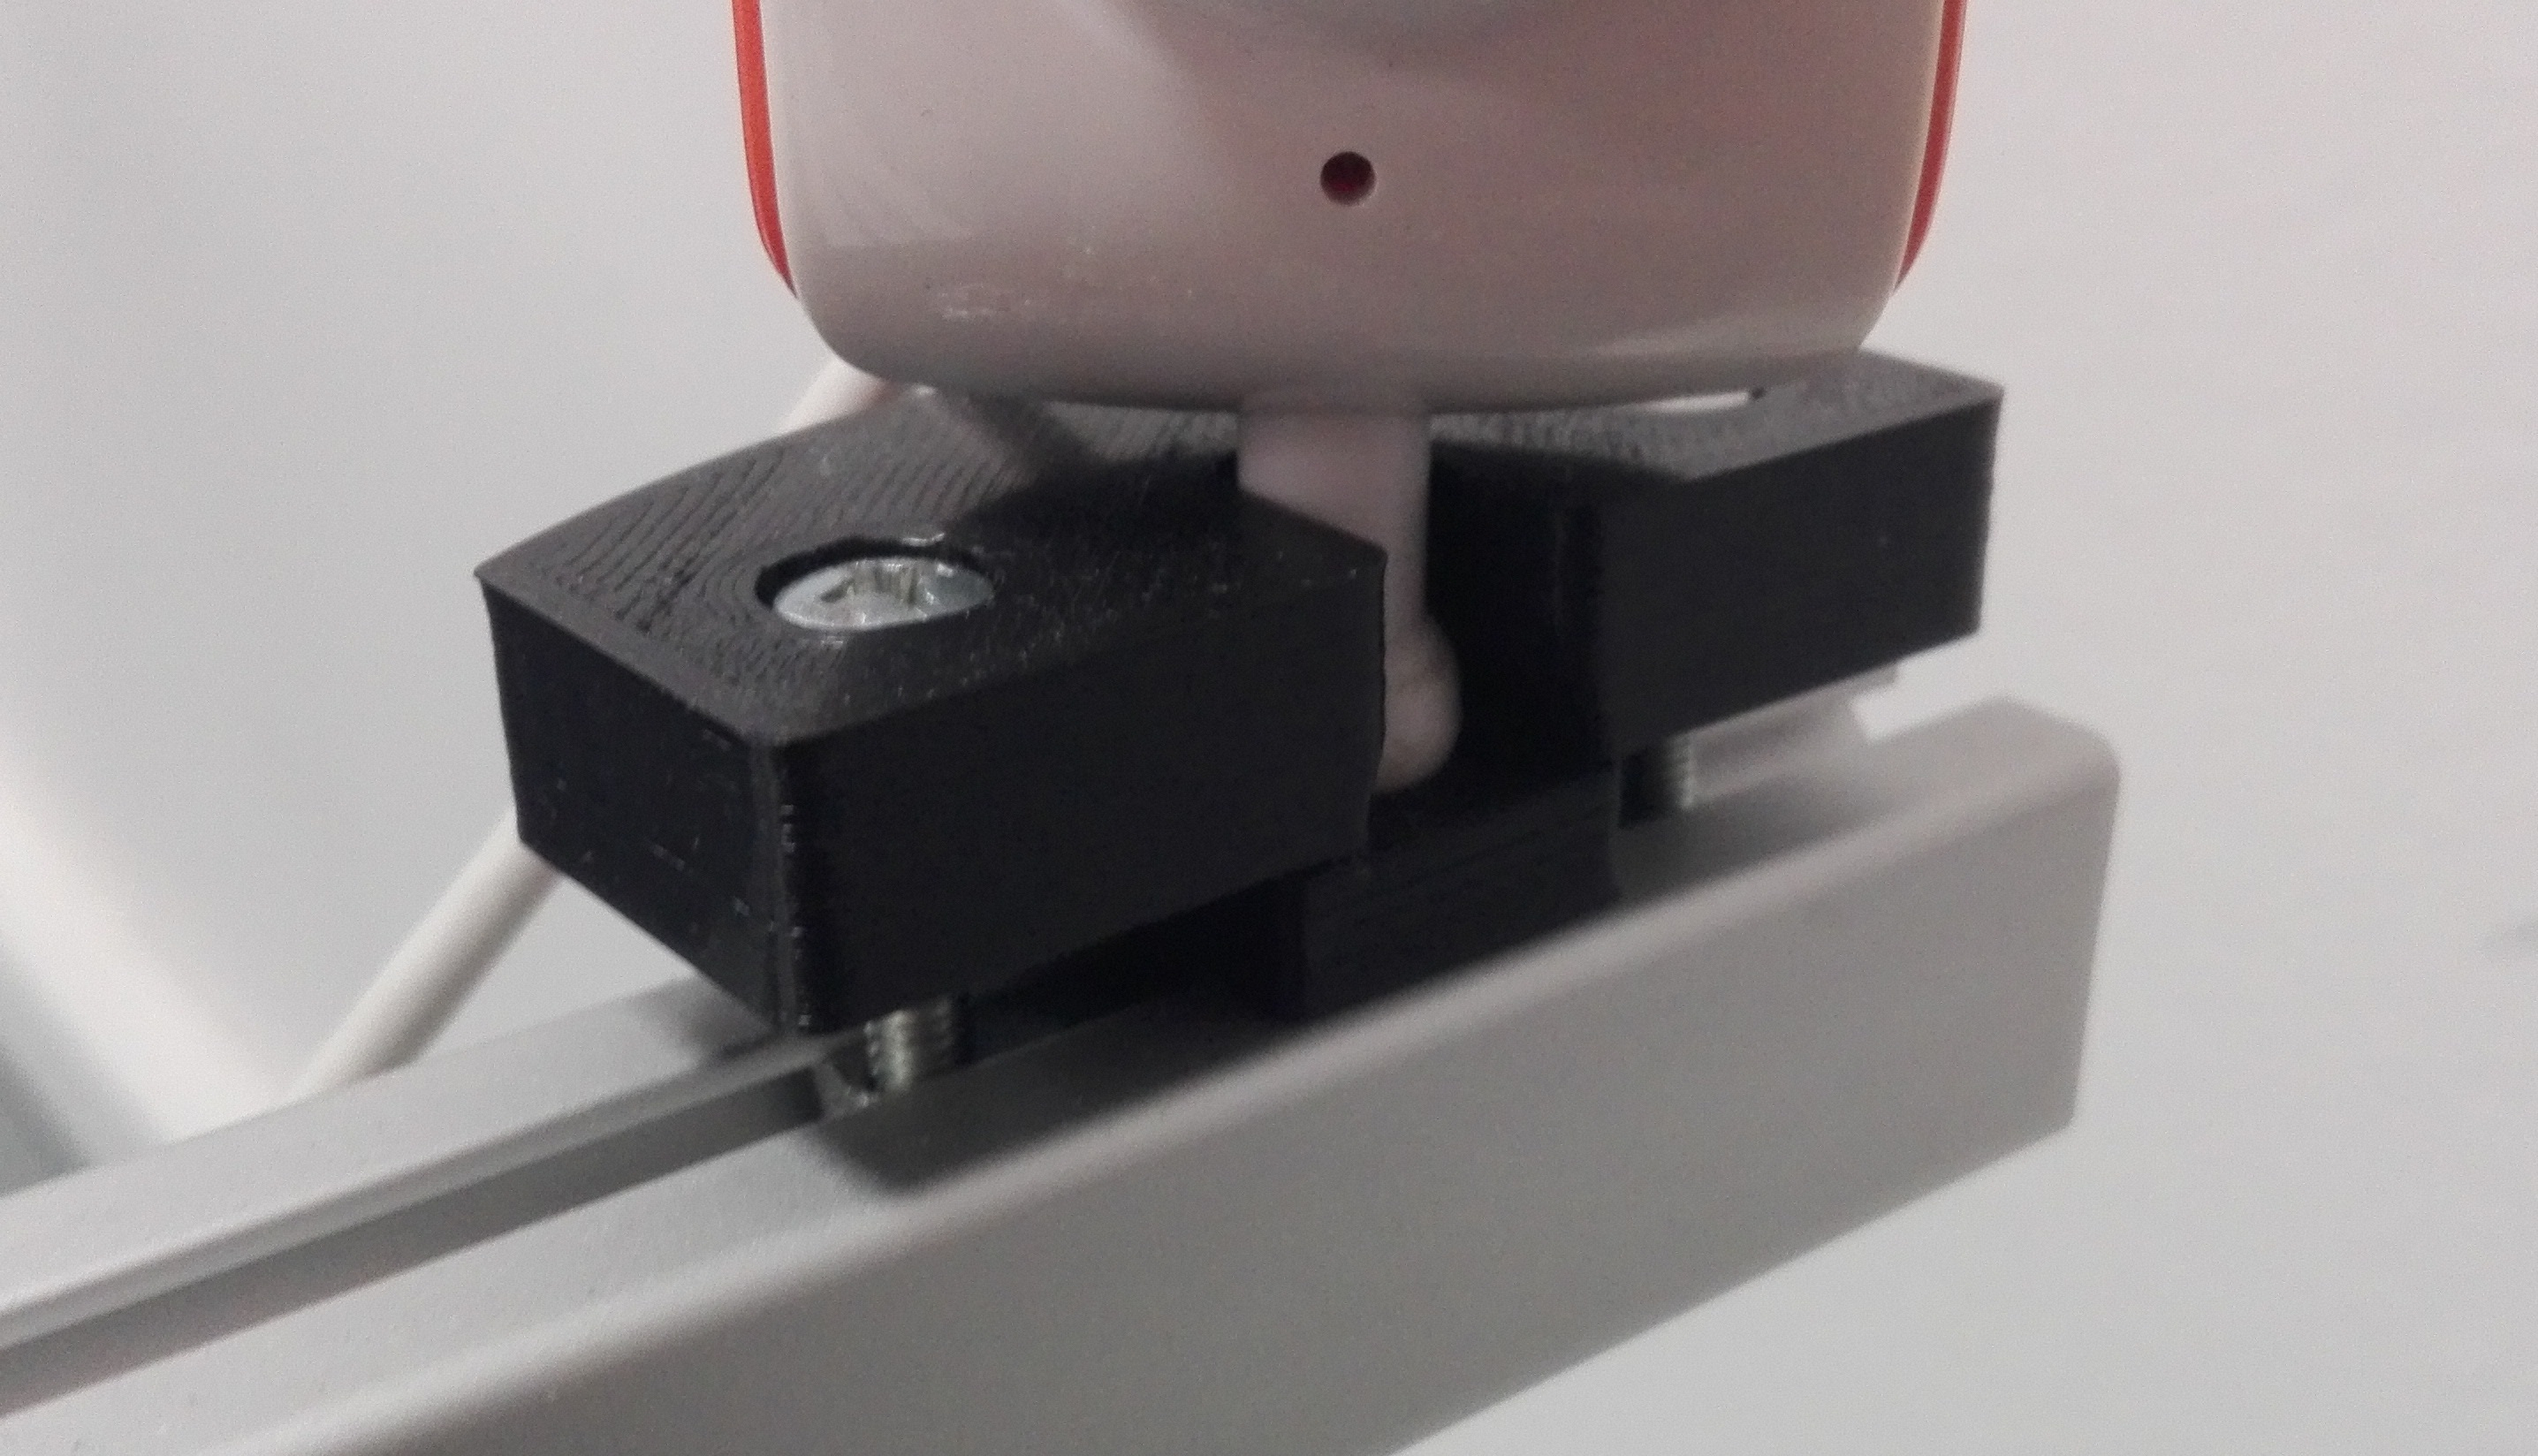
\includegraphics[height=5cm]{images/kameratarto}
	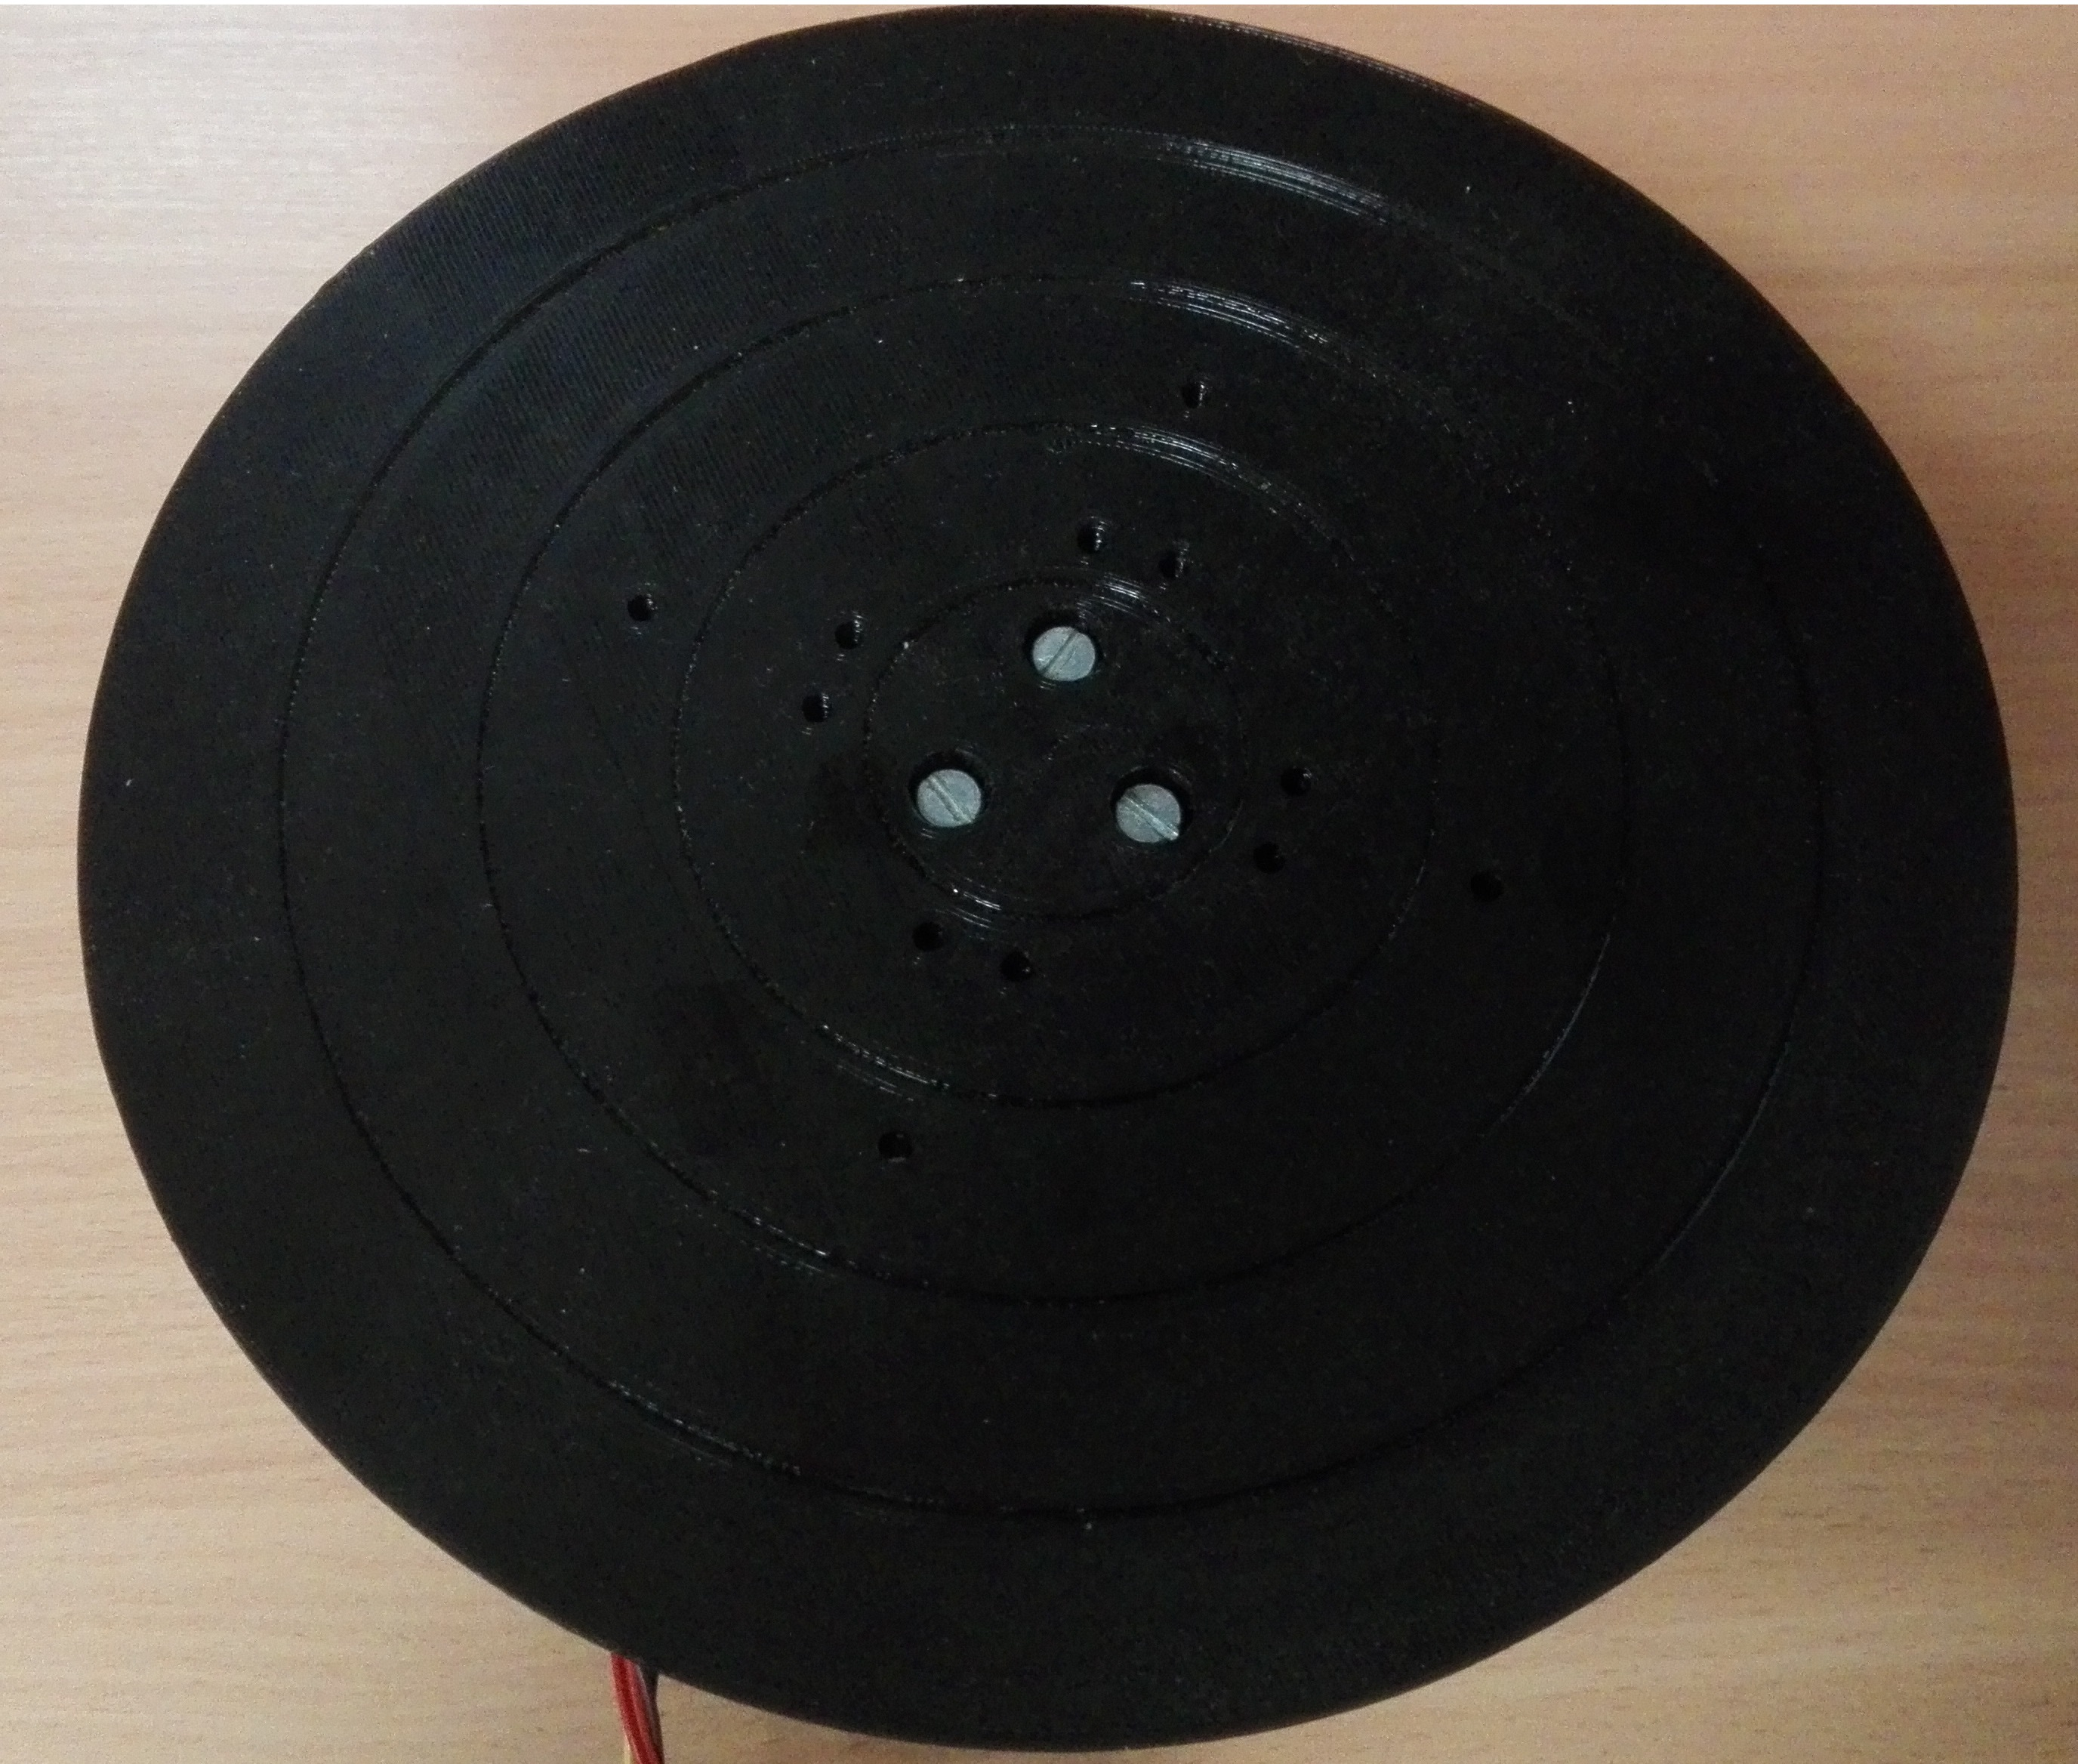
\includegraphics[height=5cm]{images/asztal}
	\caption{Saját készítésű eszközök}
\end{figure}
\subsection{Hardverek közötti csatlakozás}

Az elkészült konstrukció két részből áll. Az egyik a forgóasztal, a motor, a meghajtója és ennek vezérlő áramköre. A meghajtónak hálózati tápellátás szükséges, míg a vezérlő jelenleg számítógépről kapja az áramot USB-n keresztül.
\\[10pt]
A másik rész a kamera állvány, rajta a lézerrel és webkamerával. Utóbbi közvetlen csatlakozik a számítógéphez, míg a lézer az őt vezérlő arduino-n keresztül, szintén USB segítségével.\ref{kameraallvanyra}
\\[10pt]
Így a szkenner két részben hordozható kivitelű.\ref{hordozhatosag}
 \begin{figure}[h!]
	\centering
	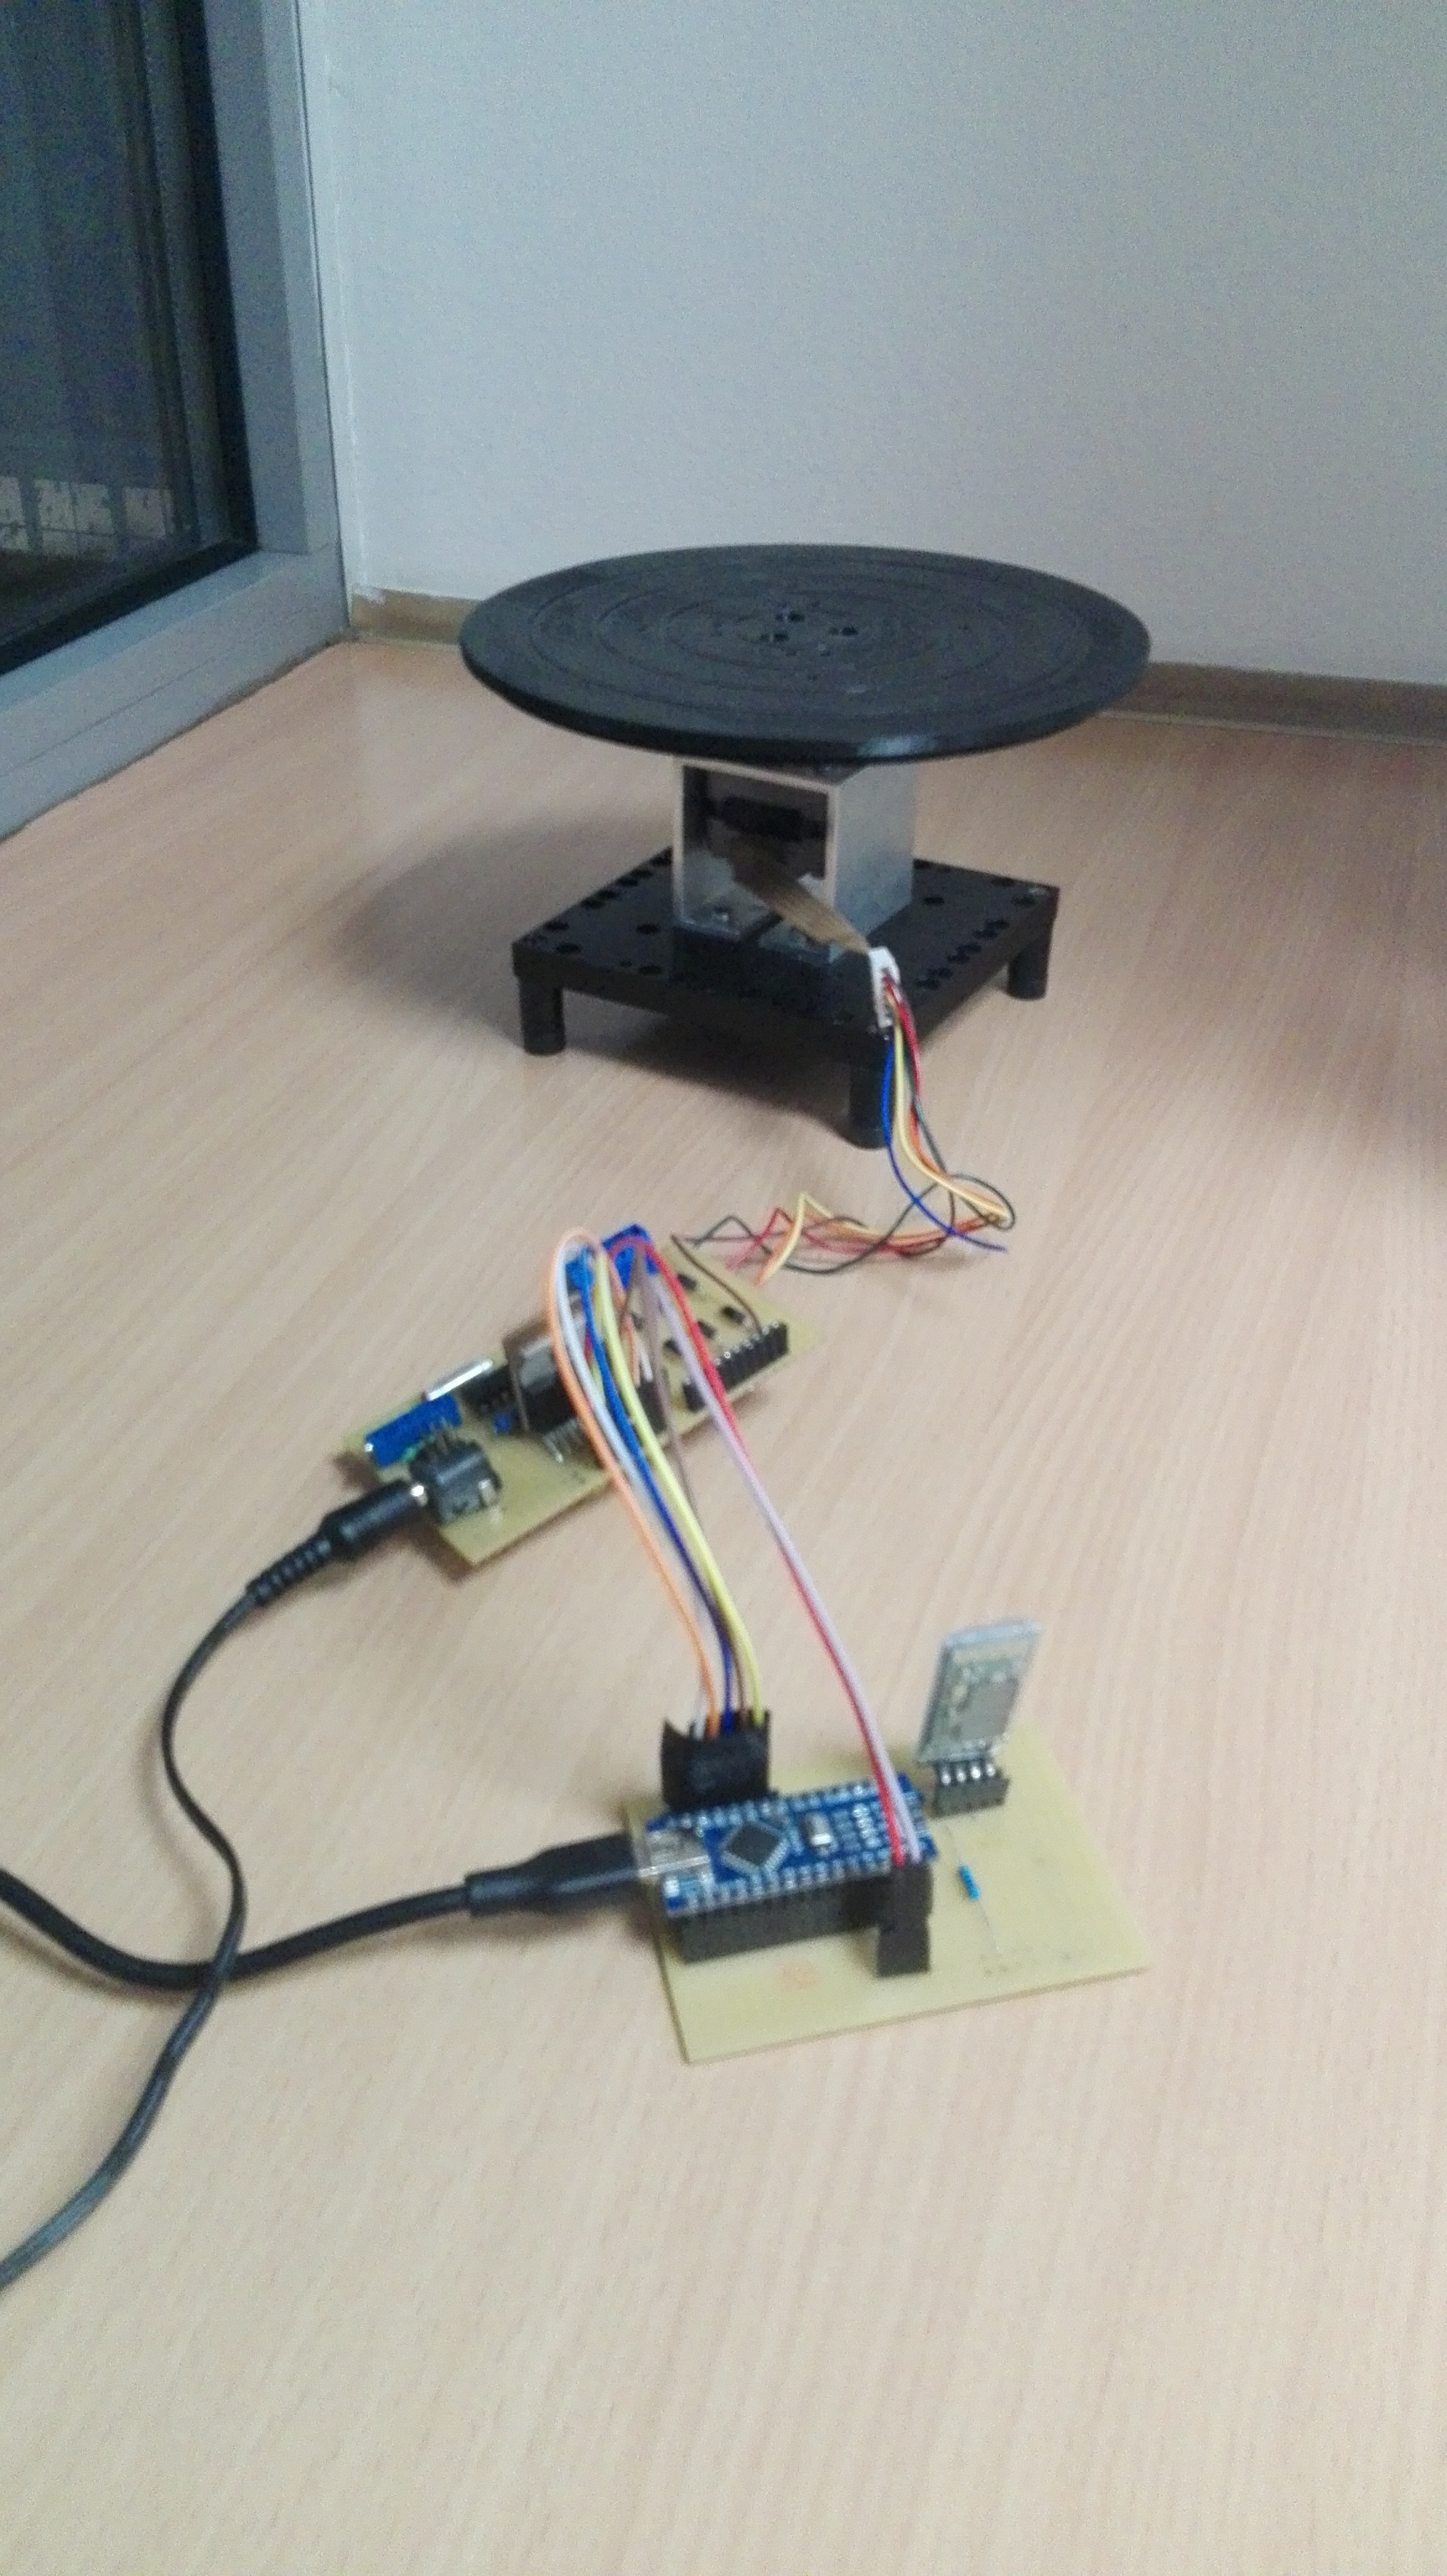
\includegraphics[width=5.5cm]{images/forgoasztal}
	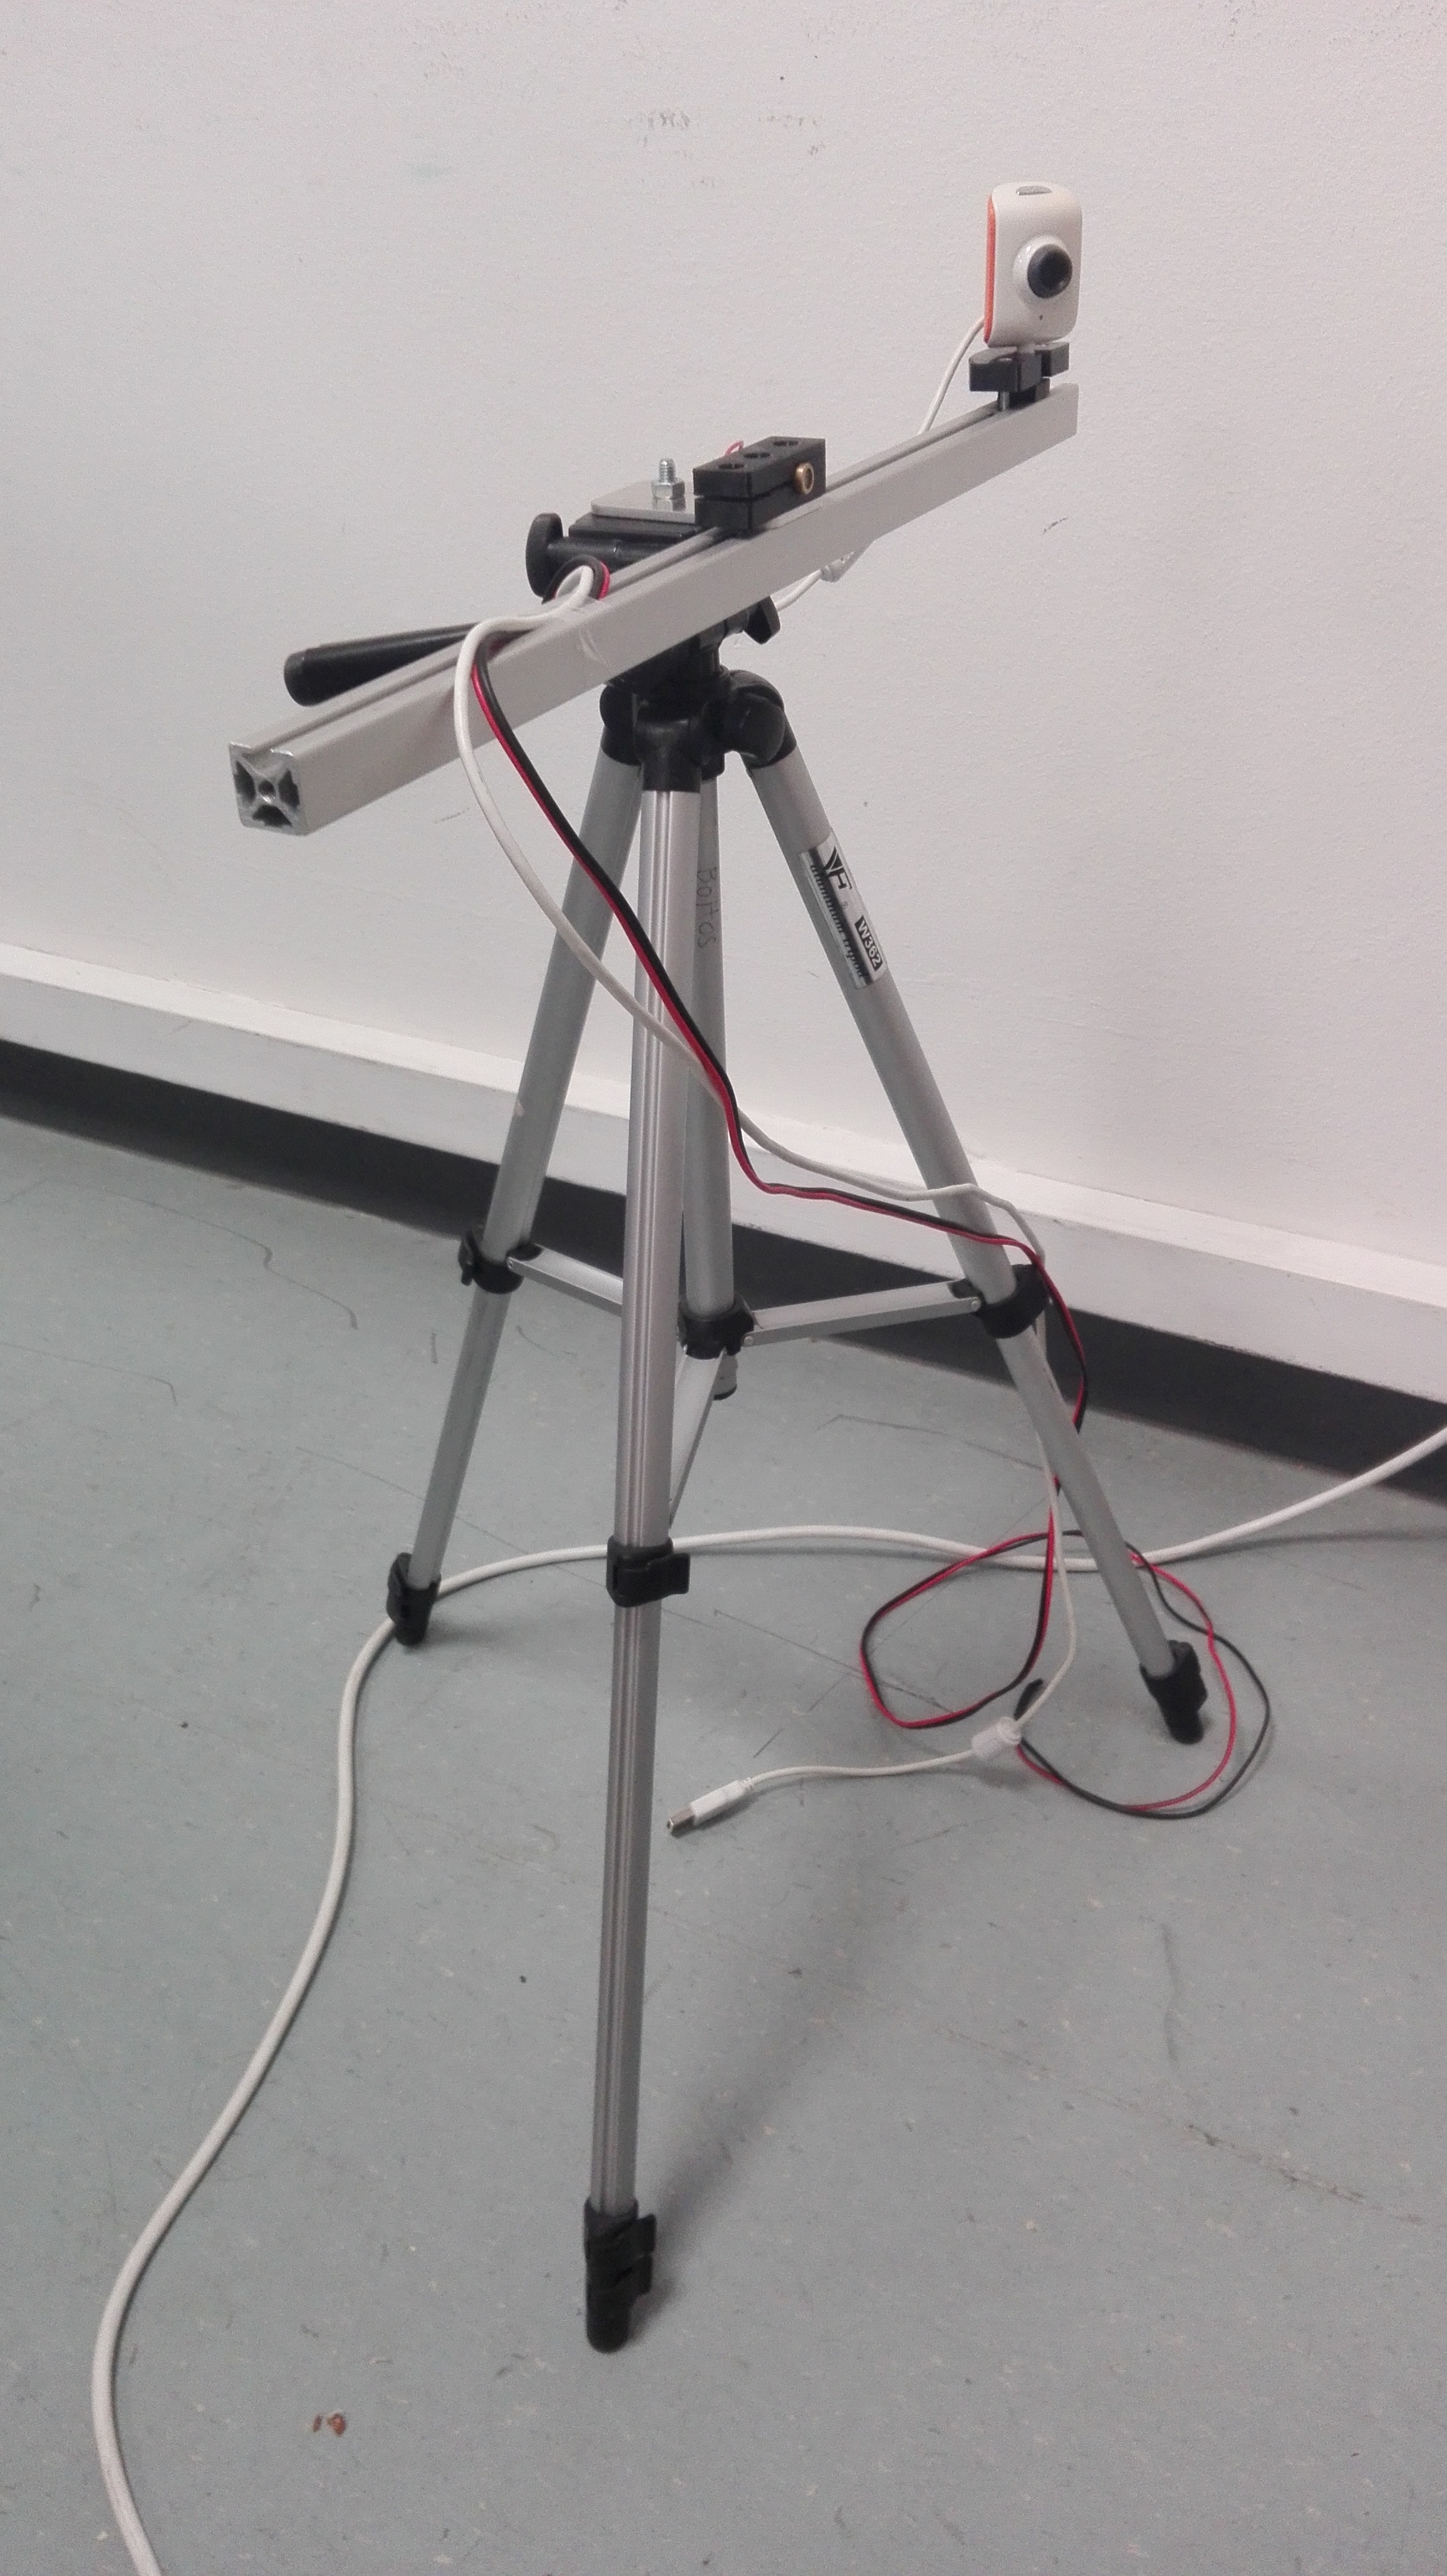
\includegraphics[width=5.5cm]{images/allvany}
	\caption{Saját készítésű eszközök}
\end{figure}
%=================================================
\section{Programkód}
Az egyes szorosan összetartozó részeket külön függvényben írtuk meg, amiket a főprogram, a scan\_object.m hív meg. A függvények csak a továbbiakban is használt változókat adják vissza, így redukáltuk a Workspace-en található vektorok számát.
\subsection{Kamera kalibráció}
\subsection{Perifériák inicializálása}
\subsection{Képek vágása}
\subsection{Transzformáció meghatározása}
\subsection{Szükséges változók deklarálása}
\subsection{Szkennelés folyamata}
\subsubsection{Lézerfény detektálása}
\subsubsection{A forgóasztal léptetése}
\subsubsection{Képek transzformációja}
\subsubsection{Pontfelhő generálása}
%=================================================
\section{Eredmények, a módszer korlátai}
%=================================================
\section{Továbbfejlesztési irányok}
%=================================================
\newpage
\begin{thebibliography}{9} 
\bibitem{feladatkiiras} 
Feladatkiírás
\href{http://mogi.bme.hu/letoltes/MECHATRONIKAI%20&%20IR%C3%81NY%C3%8DT%C3%81STECHNIKAI%20T%C3%81RGYAK/MECHATRONIKA_PROJEKT_BMEGEFOAMM3/Feladatlapok_M/}
{[link]}

\bibitem{alkalmazasok} 
3D szkennelés gyakorlati alkalmazása
\href{https://www.artec3d.com/applications}{[link]}
\texttt{http://mogi.bme.hu/letoltes/MECHATRONIKAI\%20\&\%20IR\%C3\%81NY\%C3\%8DT\%C3\%81\\
STECHNIKAI\%20T\%C3\%81RGYAK/MECHATRONIKA\_PROJEKT\_BMEGEFOAMM3/Feladatlapok\_M/}\\
2018.05.16.


%=================================================
\bibitem{FaroBuildingScan} 
\href{http://lanmarservices.com/wp-content/uploads/2014/04/Faro_Building_Scan.jpg}{Távolságmérésen alapuló lézerszkenner 1}
%=================================================
\bibitem{BridgeScan}
\href{https://i1.wp.com/cmfenews.com/wp-content/uploads/2018/04/3D-Laser.jpg?fit=1600%2C1200&ssl=1}{Távolságmérésen alapuló lézerszkenner 2}
%=================================================
\bibitem{MobileScan} 
\href{https://i.ytimg.com/vi/RVgyyIlQydg/maxresdefault.jpg}{Forgóasztalos, képfeldolgozáson alapuló 1}
%=================================================
\bibitem{PCScan}
\href{https://3dprint.com/wp-content/uploads/2015/03/Fig.-1-New-Perceptron-Smart3D-Laser-Scanning-System-3.jpg}{Forgóasztalos, képfeldolgozáson alapuló 2}
%=================================================
\bibitem{LaserScannerProjekt}
\href{http://www.instructables.com/id/3D-Laser-Scanning-DIY/}{DIY: How to Make a Low Cost 3D Scanner}
%=================================================

\end{thebibliography}

\end{document}